
\begin{figure}[ht]
    \centering
    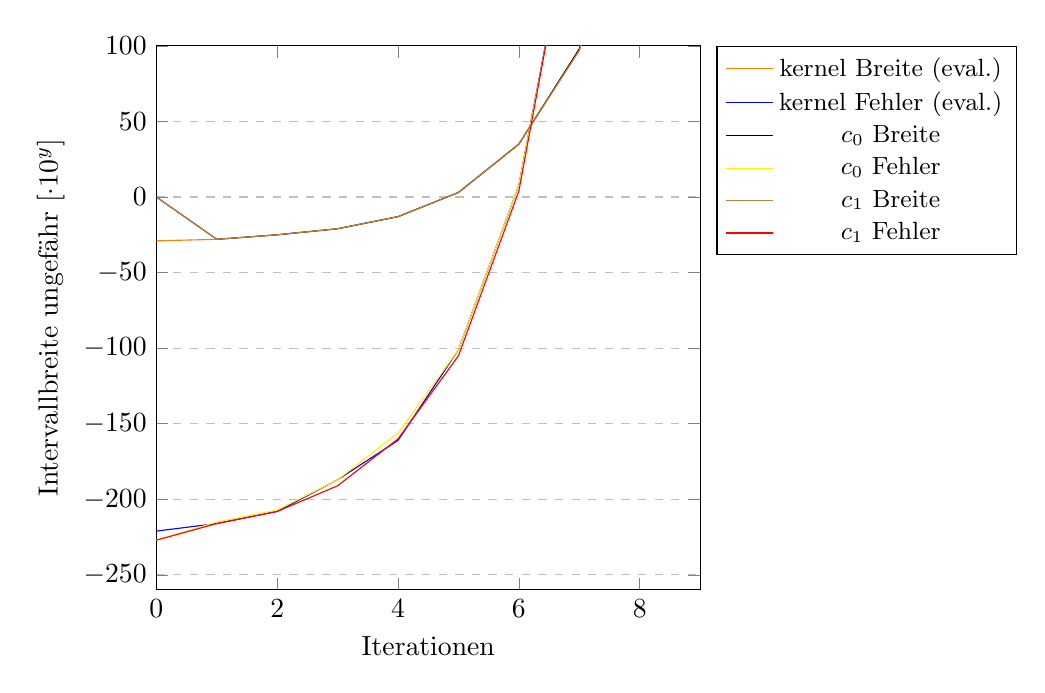
\begin{tikzpicture}
    \begin{axis}[
        width=0.7\textwidth,
        height=0.7\textwidth,
        xlabel={Iterationen},
        ylabel={Intervallbreite ungefähr $[\cdot 10^y ]$},
        legend pos=north west,
        xmin=0,xmax=9,
        ymax=100,
        ymajorgrids=true,
        grid style=dashed,
        legend pos=outer north east,
        cycle list name=color list
    ]
    
    \addplot[
        color=orange,
        ]
        coordinates {
    (0,-29)
(1,-28)
(2,-25)
(3,-21)
(4,-13)
(5,03)
(6,35)
(7,97)
(8,223)
        };
        \addlegendentry{\small{kernel Breite (eval.)}}
    
    \addplot
        coordinates {
    (0,-221)
(1,-216)
(2,-208)
(3,-187)
(4,-161)
(5,-101)
(6,8)
(7,219)
        };
        \addlegendentry{\small{kernel Fehler (eval.)}}
       
    
    \addplot
        coordinates {
    (0,0)
 (1,-28)
 (2,-25)
 (3,-21)
 (4,-13)
 (5,003)
 (6,035)
 (7,098)
 (8,223)
        };
        \addlegendentry{\small{$c_0$ Breite}}
        
    \addplot
        coordinates {
   (0,-227)
(1,-215)
(2,-207)
(3,-187)
(4,-156)
(5,-101)
(6,8)
(7,216)
(8,637)
        };
        \addlegendentry{\small{$c_0$ Fehler}}
    
        \addplot
        coordinates {
    (0,0)
 (1,-28)
 (2,-25)
 (3,-21)
 (4,-13)
 (5,+3)
 (6,+35)
 (7,+97)
 (8,+223)
        };
        \addlegendentry{\small{$c_1$ Breite}}
    
        \addplot[
        color=red,
        ]
        coordinates {
   (0,-227)
(1,-216)
(2,-208)
(3,-191)
(4,-160)
(5,-105)
(6,4)
(7,220)
        };
        \addlegendentry{\small{$c_1$ Fehler}}
    
    
    \end{axis}
    \end{tikzpicture}
    \caption{$ x_0 = [0 \pm 0] + [1 \pm 0] \cdot \lambda,\  \lambda \in [0.5 \pm \varepsilon] $}
    \label{fig:tm1}
\end{figure}